% arara: pdflatex: { synctex: yes }
% arara: makeindex: { style: ctuthesis }
% arara: bibtex

\documentclass[oneside]{ctuthesis}


%%%%%%%%%%%%%%%%%%%%%%%%%%%%%%%%%%%%%%%%%%%%%%%%%%%%%%%%%%%%%%%%%%%%%%%%%%%%%%%%
%%  ČÁST 1: ZÁKLADNÍ ÚDAJE O PRÁCI
%%  Tady se vyplňují údaje, které se objeví na titulní straně.
%%  Pozor: uvnitř \ctusetup{...} nesmí být prázdné řádky, proto jsou
%%  jednotlivé údaje oddělené jen komentáři.
%%%%%%%%%%%%%%%%%%%%%%%%%%%%%%%%%%%%%%%%%%%%%%%%%%%%%%%%%%%%%%%%%%%%%%%%%%%%%%%%

\ctusetup{
	preprint = \ctuverlog,
	mainlanguage = czech,	% pro angličtinu zvolte "english"
	doctype = M,
	specialization = S,		% {S, E, IT}
	%
	% Sem vlož název práce česky a anglicky
	title-czech = {Chytrá meteostanice s vnitřním a venkovním modulem},
	title-english = {Smart weather station with indoor and outdoor module},
	%
	% Sem vlož své jméno a jméno vedoucího práce
	author = {Martin Pinkas},
	supervisor = {Bc. Pavel Bórik},
	%
	% Sem vlož klíčová slova v češtině a v angličtině
	keywords-czech = {meteostanice, ESP32, ESP-NOW, srážkoměr, senzory, měření},
	keywords-english = {weather station, ESP32, ESP-NOW, rain gauge, sensors, measurement},
	%
	% Sem vlož datum
	day = 15,
	month = 10,
	year = 2026/2027,
}


%%%%%%%%%%%%%%%%%%%%%%%%%%%%%%%%%%%%%%%%%%%%%%%%%%%%%%%%%%%%%%%%%%%%%%%%%%%%%%%%
%%  NASTAVENÍ ŠABLONY A BALÍČKY (neupravovat)
%%  Pořadí řádků v této části je důležité.
%%%%%%%%%%%%%%%%%%%%%%%%%%%%%%%%%%%%%%%%%%%%%%%%%%%%%%%%%%%%%%%%%%%%%%%%%%%%%%%%

\usepackage[table,xcdraw, dvipsnames]{xcolor}
\usepackage{tabularray}
\usepackage{subcaption}
\usepackage{caption}
\usepackage{graphicx}
\graphicspath{{obrázky/}{./}}   % obrázky a logo se hledají ve složce obrázky (a v kořeni projektu)
\usepackage{chngcntr}
\usepackage{wrapfig}

\usepackage{url}
\usepackage{csquotes}

\ctuprocess
\hypersetup{hidelinks}
\usepackage{xurl}

\usepackage{tabularx, array, booktabs}

\addto\ctucaptionsczech{%
	\def\supervisorname{Vedoucí}%
	\def\subfieldofstudyname{Studijní program}%
}

\ctutemplateset{maketitle twocolumn default}{
	\begin{twocolumnfrontmatterpage}
		\ctutemplate{twocolumn.thanks}
		\ctutemplate{twocolumn.declaration}
		\ctutemplate{twocolumn.abstract.in.titlelanguage}
		\ctutemplate{twocolumn.abstract.in.secondlanguage}
		\ctutemplate{twocolumn.tableofcontents}
		\ctutemplate{twocolumn.listoffigures}
	\end{twocolumnfrontmatterpage}
}

\theoremstyle{plain}
\newtheorem{theorem}{Theorem}[chapter]
\newtheorem{corollary}[theorem]{Corollary}
\newtheorem{lemma}[theorem]{Lemma}
\newtheorem{proposition}[theorem]{Proposition}

\theoremstyle{definition}
\newtheorem{definition}[theorem]{Definition}
\newtheorem{example}[theorem]{Example}
\newtheorem{conjecture}[theorem]{Conjecture}

\theoremstyle{note}
\newtheorem*{remark*}{Remark}
\newtheorem{remark}[theorem]{Remark}

\setlength{\parskip}{0pt}
\setlength{\parindent}{1.25cm}

% ---------------------------------------------------------------
% Nadpisy: černý text a spojená modrá linka u nadpisů pod sebou
% ---------------------------------------------------------------
\def\ctubarup{1.0em}                        % linka nad účařím textu nadpisu (zvětšit = vyšší linka nahoru)
\def\ctubardown{0.55em}                     % linka pod účařím textu nadpisu (zvětšit = delší linka dolů)

\makeatletter
\colorlet{ctubluetext}{black}               % černé nadpisy

\newif\ifctu@isadj                          % nadpis následuje hned po jiném nadpisu
\newskip\ctu@after
\newdimen\ctu@up
\newdimen\ctu@dn
\newdimen\ctu@tnow
\newdimen\ctu@tprev
\newdimen\ctu@dprev
\newdimen\ctu@gap
\newdimen\ctu@ovl
\newdimen\ctu@ovlup
\ctu@ovl=1pt                                % přesah spojovací linky dovnitř spodního nadpisu
\ctu@ovlup=3pt                              % přesah spojovací linky nahoru do horního nadpisu (kryje případnou škvíru)

% zjistí, jestli nadpis následuje hned po nadpisu, a zruší mezeru mezi nimi
\def\ctu@pre{%
	\if@nobreak\ctu@isadjtrue\else\ctu@isadjfalse\fi
	\ifctu@isadj
		\nobreak                              % mezi dvěma nadpisy nesmí být konec strany
		\vskip-\ctu@after
		\prevdepth=-\maxdimen
	\fi
}

% #1 písmo nadpisu, #2 obsah nadpisu
\long\def\ctu@hbar#1#2{%
	\setbox\ctu@title@box\vtop{%
		\hsize\dimexpr\linewidth-\ctu@title@rulewidth-\ctu@title@rulesep\relax
		\linespread{1}\selectfont              % řádkování 1,5 se u nadpisů nepoužije
		\sffamily\bfseries\raggedright
		#1\relax
		\global\ctu@up=\ctubarup\relax
		\global\ctu@dn=\ctubardown\relax
		\noindent\strut #2\strut\par
	}%
	% víceřádkový nadpis: linka musí sahat i pod poslední řádek
	\ifdim\dimexpr\dp\ctu@title@box+0.15\ctu@up\relax>\ctu@dn
		\ctu@dn=\dimexpr\dp\ctu@title@box+0.15\ctu@up\relax
	\fi
	\ifctu@isadj\nobreak\fi                  % ani těsně před druhým nadpisem nesmí být konec strany
	\noindent\hbox{%
		{\color{Automatizace}\rule[-\ctu@dn]{\ctu@title@rulewidth}{\dimexpr\ctu@up+\ctu@dn\relax}}%
		\hspace*{\ctu@title@rulesep}%
		\raisebox{0pt}[0pt][0pt]{\box\ctu@title@box}%
	}\par
	\ctu@tnow=\pagetotal
	\ifctu@isadj
		% doplní linku mezi dvěma nadpisy pod sebou
		\ctu@gap=\dimexpr\ctu@tnow-\ctu@up-\ctu@tprev-\ctu@dprev\relax
		\ifdim\ctu@gap>-30pt\ifdim\ctu@gap<60pt
			\ifdim\ctu@gap<0pt\ctu@gap=0pt\fi
			\dimen@ii=\prevdepth
			\nointerlineskip
			\vbox to 0pt{\vss\hbox to 0pt{\raisebox{\dimexpr\ctu@up+\ctu@dn-\ctu@ovl\relax}[0pt][0pt]{\color{Automatizace}\rule{\ctu@title@rulewidth}{\dimexpr\ctu@gap+\ctu@ovl+\ctu@ovlup\relax}}\hss}}%
			\prevdepth=\dimen@ii
		\fi\fi
	\fi
	\global\ctu@tprev=\ctu@tnow
	\global\ctu@dprev=\ctu@dn
	\global\ctu@after=\@tempskipb
	\nobreak                                  % nadpis se neoddělí od toho, co následuje
}

\def\ttlh@ctuch#1#2#3#4#5#6#7#8{%
	\ctu@pre
	\ifttl@label\else\chapterstarmark{#8}\fi
	\ifttl@label\else\addcontentsline{toc}{chapter}{#8}\fi
	\ctu@hbar{#4}{\ifttl@label\thechapter\quad\fi#8}%
}
\def\ttlh@ctus#1#2#3#4#5#6#7#8{%
	\ctu@pre
	\ifttl@label\else\sectionstarmark{#8}\fi
	\ifttl@label\else\addcontentsline{toc}{section}{#8}\fi
	\ctu@hbar{#1}{\ifttl@label#2\fi\color{ctubluetext}#8}%
}
\def\ttlh@ctuss#1#2#3#4#5#6#7#8{%
	\ctu@pre
	\ifttl@label\else\addcontentsline{toc}{subsection}{#8}\fi
	\ctu@hbar{#1}{\ifttl@label#2\fi\color{ctubluetext}#8}%
}
\def\ttlh@ctusss#1#2#3#4#5#6#7#8{%
	\ctu@pre
	\ifttl@label\else\addcontentsline{toc}{subsubsection}{#8}\fi
	\ctu@hbar{#1}{\ifttl@label#2\fi\color{ctubluetext}#8}%
}
\titlespacing*{\chapter}{0pt}{0pt}{20pt}
\makeatother


%%%%%%%%%%%%%%%%%%%%%%%%%%%%%%%%%%%%%%%%%%%%%%%%%%%%%%%%%%%%%%%%%%%%%%%%%%%%%%%%
%%  ČÁST 2: ÚVODNÍ STRANY PRÁCE
%%  Na prázdný řádek před \end{...} piš text.
%%%%%%%%%%%%%%%%%%%%%%%%%%%%%%%%%%%%%%%%%%%%%%%%%%%%%%%%%%%%%%%%%%%%%%%%%%%%%%%%

% Sem vlož poděkování
\begin{thanks}
	Diky.
	\end{thanks}


% Sem vlož prohlášení
\begin{declaration}
prohlasuju ze nebudu podvadet.

\noindent Nemám závažný důvod proti užití tohoto školního díla ve smyslu §\,60 zákona č.~121/2000 Sb., o~právu autorském, o~právech souvisejících s~právem autorským a o~změně některých zákonů (autorský zákon).

\noindent V Praze, říjen 2026

\vskip1cm
\noindent\dotfill
\begin{center}Podpis autora práce\end{center}

\end{declaration}


% Sem vlož abstrakt v češtině
\begin{abstract-czech}
Práce se zabývá návrhem, sestavením a naprogramováním chytré meteostanice s vnitřním a venkovním modulem. Venkovní modul měří teplotu, vlhkost, vítr a srážky, vnitřní modul navíc tlak a zobrazuje všechna data na dotykovém displeji. Moduly komunikují bezdrátově pomocí ESP-NOW a data jsou dostupná i online.

\end{abstract-czech}


% Sem vlož abstrakt v angličtině
\begin{abstract-english}
This thesis covers the design, construction and programming of a smart weather station with an indoor and an outdoor module. The outdoor module measures temperature, humidity, wind and precipitation, while the indoor module also measures pressure and shows all data on a touchscreen. The modules communicate wirelessly using ESP-NOW and the data is also available online.

\end{abstract-english}


%%%%%%%%%%%%%%%%%%%%%%%%%%%%%%%%%%%%%%%%%%%%%%%%%%%%%%%%%%%%%%%%%%%%%%%%%%%%%%%%
%%  ČÁST 3: VLASTNÍ DOKUMENT
%%  Zadání, kapitoly a zdroje.
%%%%%%%%%%%%%%%%%%%%%%%%%%%%%%%%%%%%%%%%%%%%%%%%%%%%%%%%%%%%%%%%%%%%%%%%%%%%%%%%

\begin{document}
	\maketitle

	% Řádkování 1,5 od úvodu dál (před titulní stranou by zvětšilo logo)
	\linespread{1.5}\selectfont

	% Sem vlož zadání práce (soubor zadani.pdf nahraj do projektu)
	% \includepdf[pages=-]{zadani.pdf}

	% Sem vlož jednotlivé kapitoly, každá je v samostatném souboru
	\chapter * {Úvod}

Měření počasí přímo v~místě, kde ho potřebujeme znát, je užitečné například při práci na zahradě nebo při rozhodování o~zalévání. Údaje z~veřejných předpovědí a vzdálenějších stanic totiž nemusí odpovídat tomu, co se děje u~konkrétního domu. Tato práce se zabývá návrhem, stavbou a naprogramováním chytré meteostanice, která tyto údaje měří přímo na místě. Skládá se z~venkovního modulu, který měří teplotu, vlhkost, vítr, srážky a intenzitu osvětlení, a z~vnitřního modulu, který tato data přijímá, doplňuje je o~vlastní měření teploty, vlhkosti a tlaku a zobrazuje je uživateli.

Práci zpracovávám jako maturitní práci a hlavním důvodem, proč jsem si vybral právě meteostanici, je možnost získat při jejím vypracování praktické zkušenosti. Projekt spojuje mechanickou konstrukci, elektroniku i programování, takže si na něm mohu vyzkoušet celý postup od návrhu až po funkční zařízení. Zároveň se dá rozdělit na samostatné části, jako je venkovní modul, vnitřní modul, komunikace mezi nimi a software, které lze postupně navrhovat, vyrábět a testovat. Na trhu je řada hotových meteostanic, které jsou kvalitně zpracované a nabízejí více, než dokážu vytvořit já. Nechci proto vytvořit lepší zařízení, ale ověřit si, že podobné řešení dokážu samostatně navrhnout, postavit a uvést do provozu.

Cílem práce je navrhnout, sestavit a naprogramovat funkční prototyp meteostanice, který měří teplotu, vlhkost, tlak, intenzitu osvětlení, rychlost a směr větru a úhrn srážek. Naměřené hodnoty a jejich historie se zobrazují na displeji a~na webové stránce a součástí zařízení je také jednoduché doporučení k~zavlažování. Funkce zařízení ověřuji v~reálných podmínkách. Největším přínosem práce jsou pro mě zkušenosti, které získám při řešení konkrétních problémů při návrhu, výrobě a oživení zařízení. Součástí práce je také technická dokumentace.
	\chapter{Měření srážek}

\section{Požadavky}

Srážkoměr bude součástí venkovního modulu, takže musí fungovat dlouhodobě venku a~jeho signál musí zpracovat mikrokontrolér. Naměřená data se použijí pro 15minutové souhrny, pro denní a~týdenní přehled srážek a~pro jednoduché doporučení zálivky, proto musí být měření stabilní a~opakovatelné. Zařízení se musí dát snadno zapojit a~naprogramovat, mělo by jít objednat z~evropského obchodu a~výhodou je také dostupná dokumentace.

\section{Principy měření}

\subsection{Kyvný kyblík}

Nejrozšířenějším principem je kyvný kyblík (anglicky \textit{tipping bucket}). Voda ze sběrné nálevky teče do kyvné nádobky se dvěma komorami. Jakmile se jedna komora naplní na určitý objem, nádobka se převrátí, voda vyteče a~plnit se začne druhá komora. Při každém převrácení se pomocí magnetu sepne jazýčkový kontakt, který vytvoří jeden impuls. Jeden impuls tak odpovídá pevně dané výšce srážek. U~srážkoměrů pro malé meteostanice to je například 0,2794~mm na jedno překlopení~\cite{sparkfun}, jiný výrobce ale uvádí 0,3~mm~\cite{misol}.

Princip je znázorněn na obrázku~\ref{fig:kyblik}.

\begin{figure}[htbp]
\centering
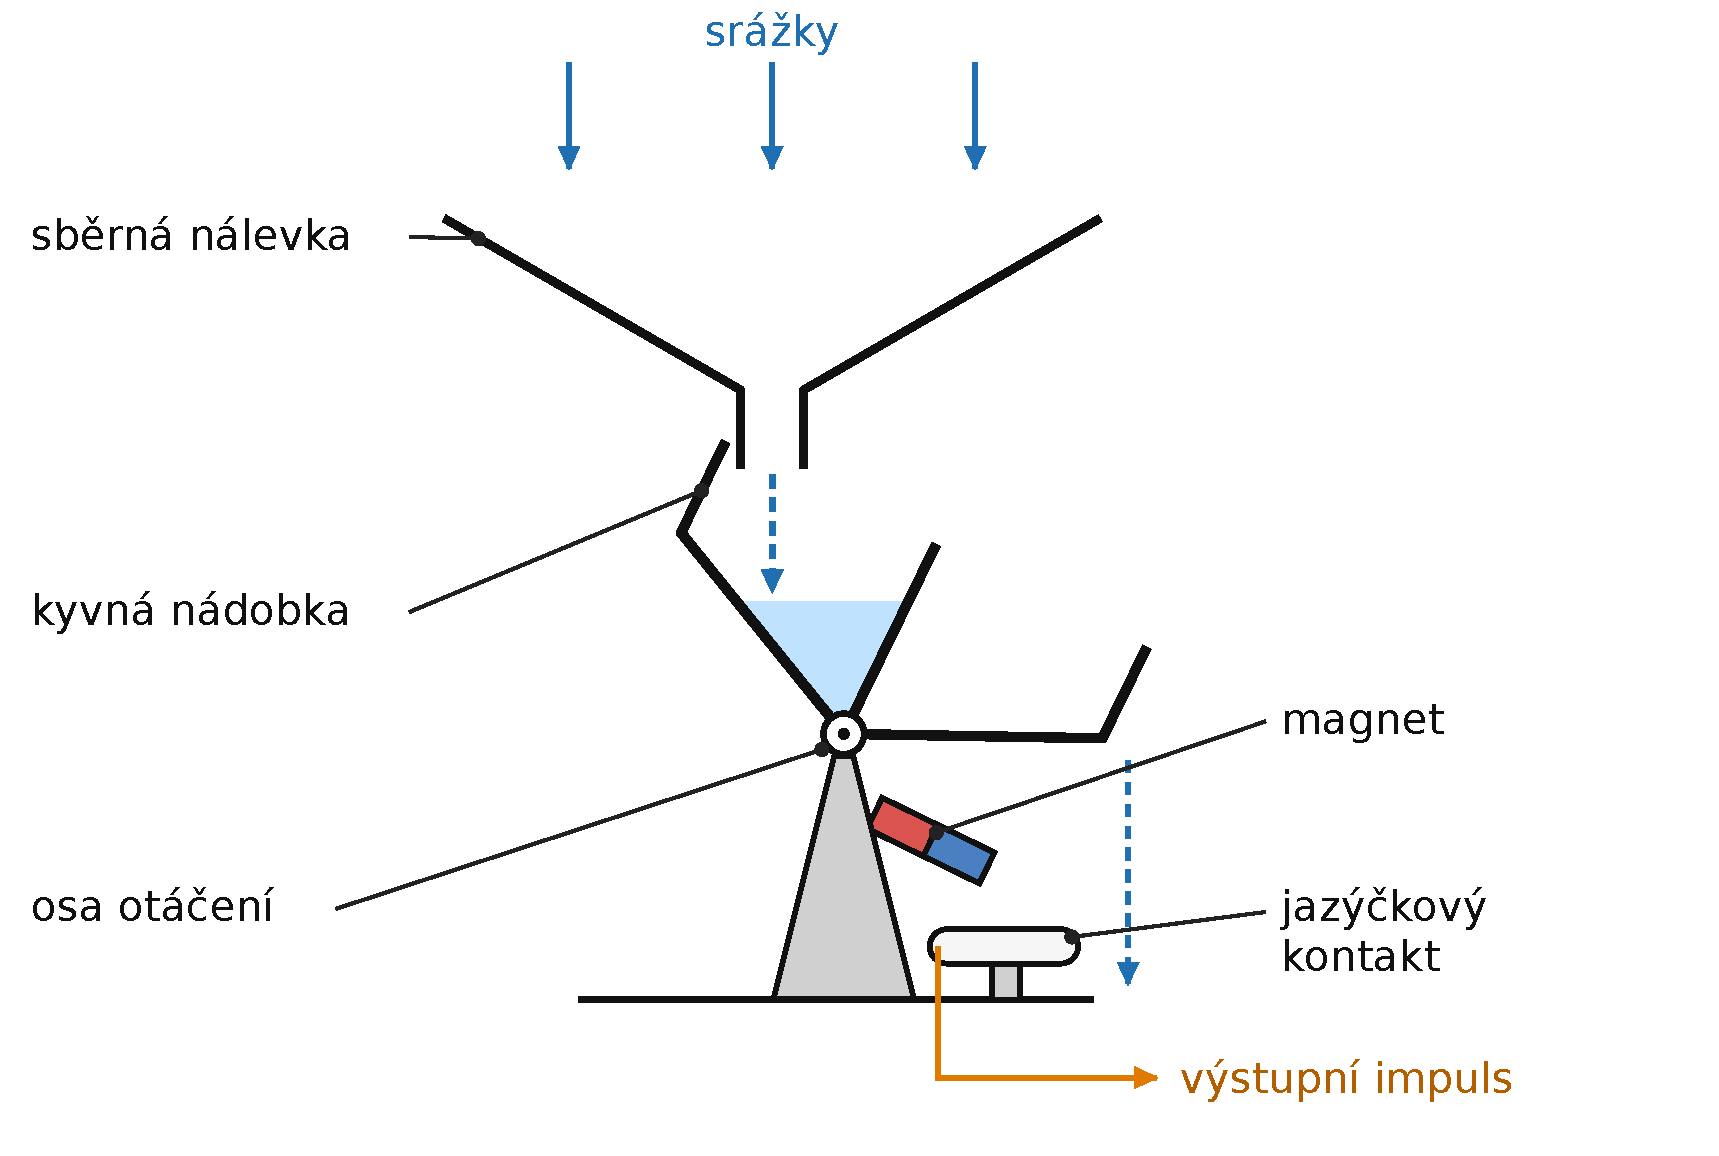
\includegraphics[width=0.8\textwidth]{kyvny_kyblik}
\caption{Princip srážkoměru s~kyvným kyblíkem}
\label{fig:kyblik}
\end{figure}

Výstup je pro mikrokontrolér velmi jednoduchý. Kontakt neobsahuje žádnou aktivní elektroniku a~stačí ho připojit na vstup s~přerušením a~počítat impulsy~\cite{sparkfun}. Tímto způsobem je řešený například srážkoměr v~diplomové práci o~domácí meteostanici, kde mikrokontrolér ESP32 počítá překlopení v~přerušení~\cite{macek}. Základní provedení srážkoměru není vytápěné, takže měří jen kapalné srážky, vytápění umožňuje měřit i sníh~\cite{macek}.

\subsection{Váhový princip}

Při váhovém principu se voda zachycuje do nádoby a~její hmotnost se měří snímačem síly. Výška srážek se dopočítá z~hmotnosti vody a~plochy nálevky, protože 1~mm srážek odpovídá 1~kg vody na metr čtvereční. Při sběrné ploše 200~cm$^2$ tedy 1~mm srážek odpovídá 20~g vody a~0,2~mm odpovídá 4~g. Typickým profesionálním příkladem je OTT Pluvio$^2$ S, který váží uzavřeným snímačem síly, má sběrnou plochu 200~cm$^2$, kapacitu 400~mm a~přesnost $\pm$0,1~mm nebo $\pm$1~\% naměřené hodnoty. Váží kolem 7,8~kg a~je určený pro profesionální použití~\cite{ott}.

Jako možnost vlastní stavby by šlo postavit váhový srážkoměr s~tenzometrickým snímačem. Voda z~nálevky by se zachytávala do nádoby, jejíž hmotnost by se měřila a~digitalizovala 24bitovým převodníkem HX711~\cite{hx711}. Nádoba by se vyprazdňovala posuvným šoupátkem poháněným servem. U~takového konceptu je potřeba řešit vyprazdňování nádoby tak, aby nezkreslovalo vážení, a~počítat také s~pohybem konstrukce při větru.

Koncept je znázorněn na obrázku~\ref{fig:vahovy}.

\begin{figure}[htbp]
\centering
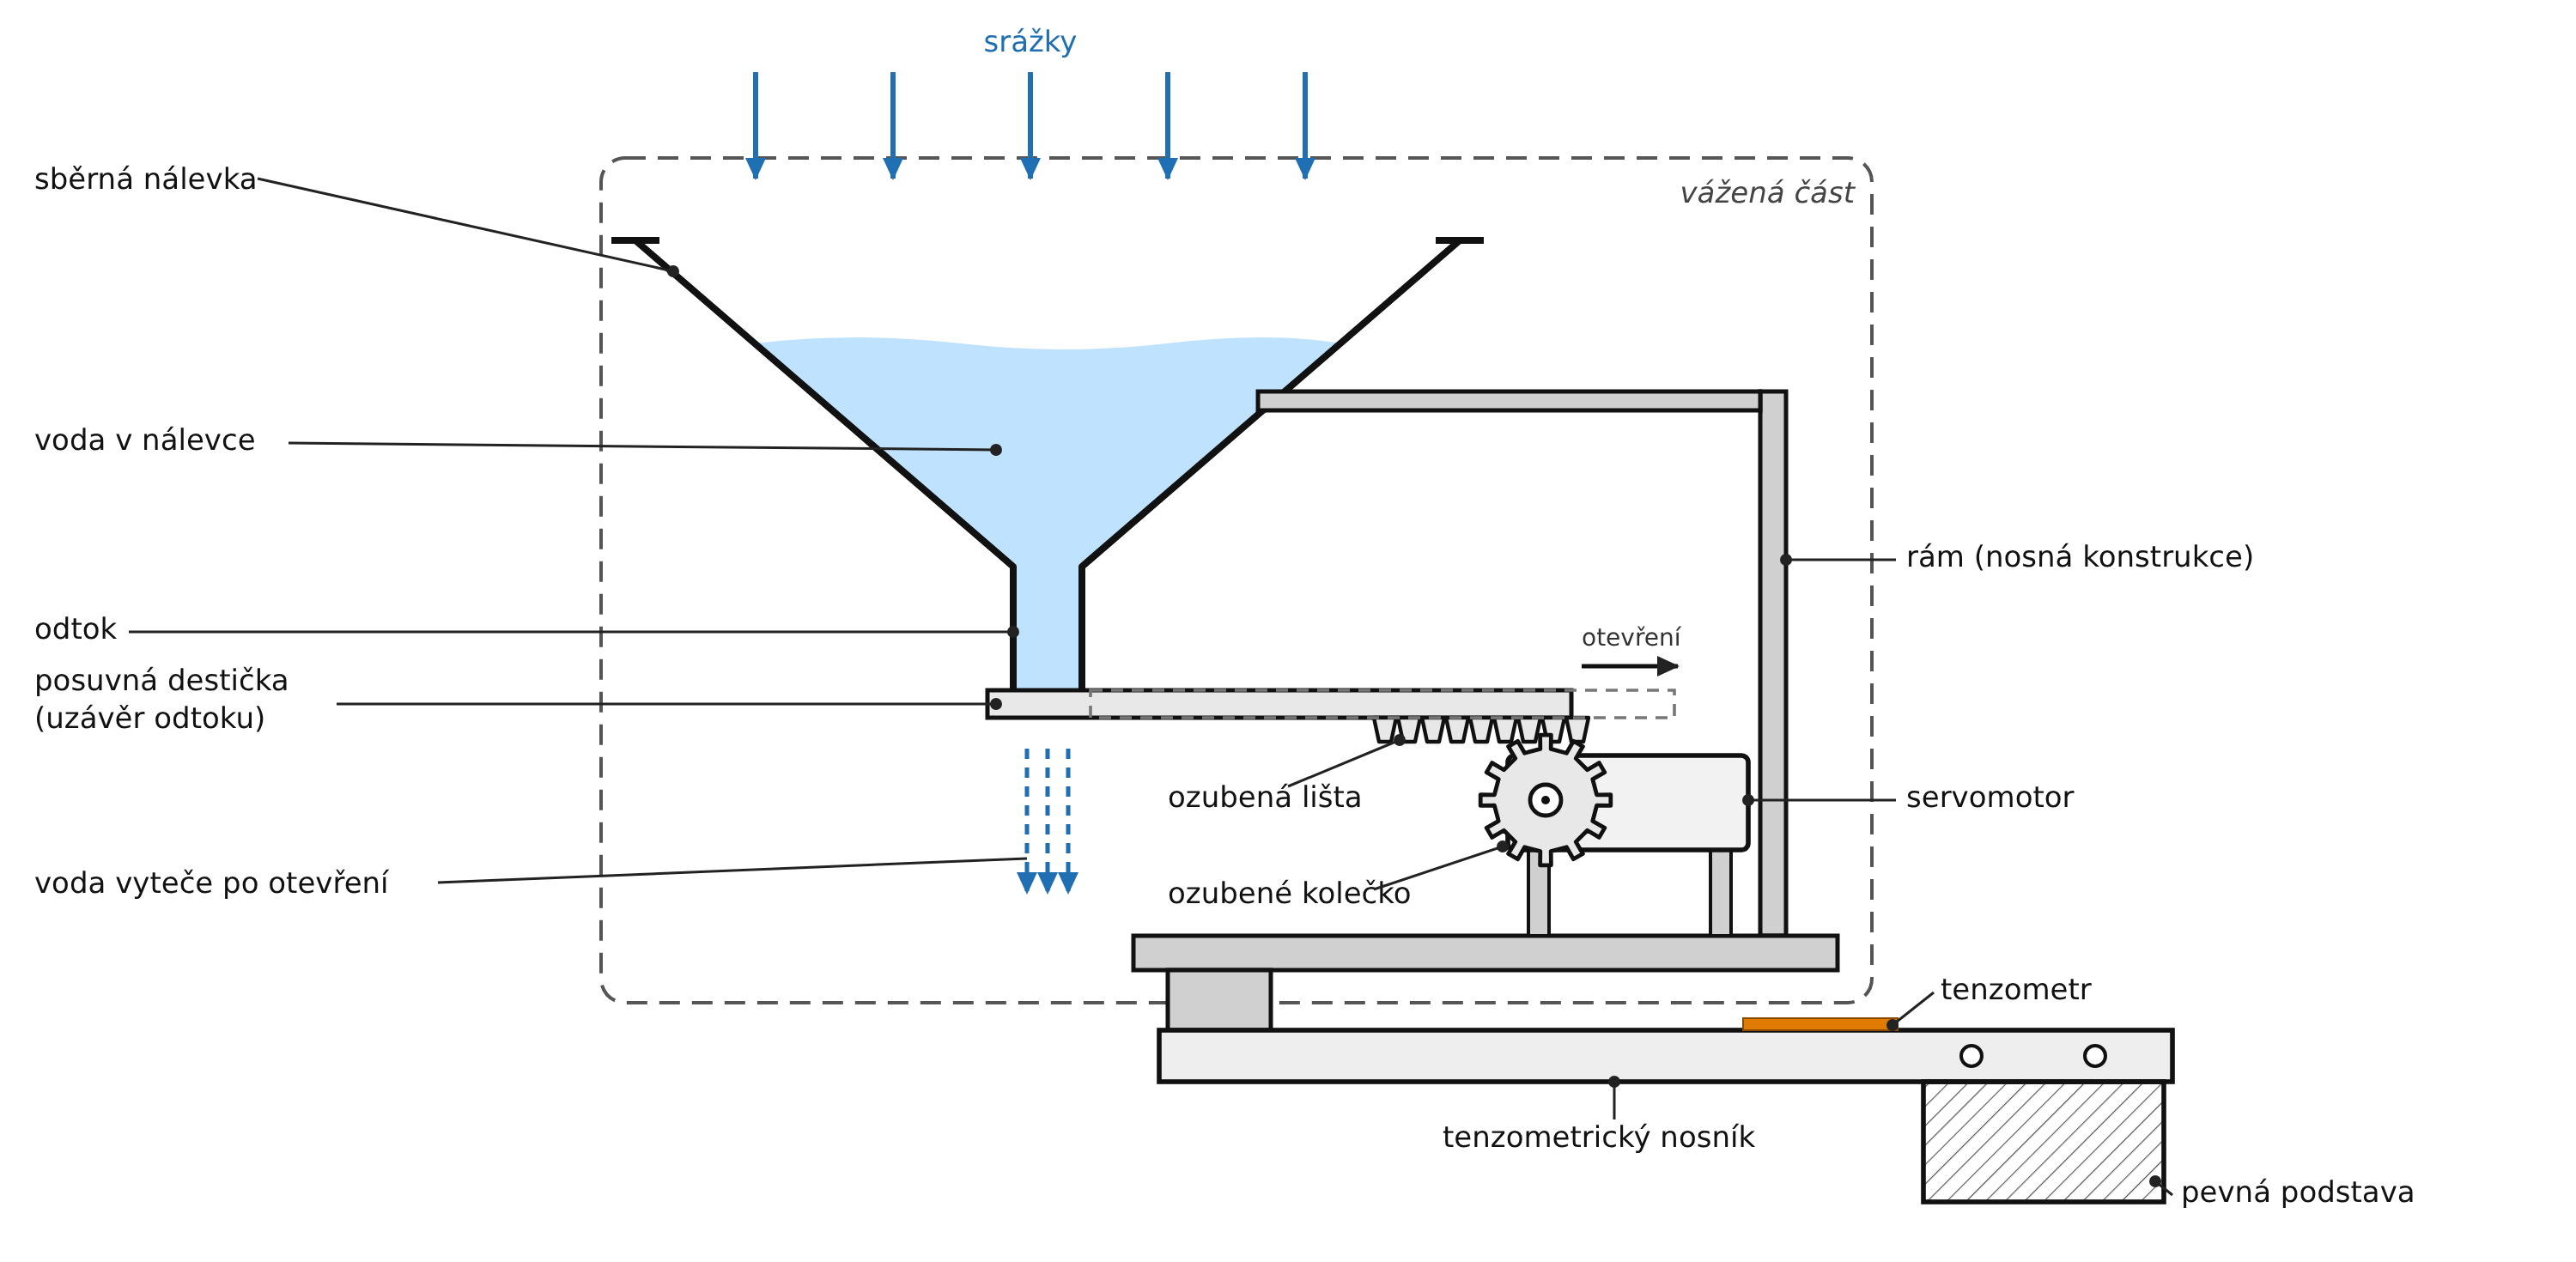
\includegraphics[width=\textwidth]{vahovy_srazkomer}
\caption{Koncept váhového srážkoměru s~tenzometrem}
\label{fig:vahovy}
\end{figure}

\subsection{Optické a~další principy}

Optický srážkoměr nesbírá vodu, ale srážky odhaduje. Infračervené světlo se uvnitř čočky odráží k~detektorům a~kapky dopadající na povrch čočky způsobí, že část světla uniká ven. Z~poklesu intenzity se odhadne velikost kapek a~z~nich množství srážek~\cite{cnx}. Příkladem je Hydreon RG-15, který nemá žádné pohyblivé části. V~klidu spotřebuje asi 110~$\mu$A, za deště 2 až 4~mA. Jeho výstup napodobuje kyblík a~je k~dispozici i~sériové rozhraní. Nominální přesnost je $\pm$10~\%, výrobce uvádí, že se v~terénu může lišit, a~při mrznoucím dešti senzor srážky nezaznamená~\cite{rg15}. Existují i~další principy, například piezoelektrické nebo radarové, ty se ale používají hlavně v~komplexnějších čidlech.

\section{Porovnání principů}

Tabulka~\ref{tab:srazky} shrnuje hlavní vlastnosti popsaných principů a~konkrétních řešení.

\newcolumntype{Y}[1]{>{\hsize=#1\hsize\raggedright\arraybackslash}X}

\begin{center}
\noindent\begin{minipage}{\textwidth}
\captionof{table}{Porovnání principů a~konkrétních řešení měření srážek}
\label{tab:srazky}
\scriptsize
\renewcommand{\arraystretch}{1.25}
\begin{tabularx}{\textwidth}{|Y{1.5}|Y{0.8}|Y{0.8}|Y{0.9}|}
\hline
\textbf{Řešení} & \textbf{Rozlišení} & \textbf{Přesnost} & \textbf{Výstup} \\
\hline
\rowcolor{gray!15}\multicolumn{4}{|l|}{\textbf{Kyvný kyblík}} \\
\hline
HESTORE WH-SP-RG (plast) & 0,2794~mm & $\pm$5~\% & kontakt \\
\hline
Davis 6466M (UV-ABS) & 0,2~mm & $\pm$3~\% & kontakt \\
\hline
Rika RK400-01 (nerez, ABS) & 0,2~mm & $\pm$4~\% & kontakt, RS485 \\
\hline
Veinasa XS-RS04 (nerez) & 0,2~mm & $\pm$4~\% & kontakt \\
\hline
BGT WS-601 SS (nerez) & 0,2~mm & $\pm$2~\% & kontakt, RS485 \\
\hline
\rowcolor{gray!15}\multicolumn{4}{|l|}{\textbf{Váhový}} \\
\hline
OTT Pluvio$^2$ S (7,8~kg) & 0,05 až 0,2~mm & $\pm$1~\% & impulsy, SDI-12, RS-485 \\
\hline
Vlastní koncept (tenzometr, HX711) & dáno snímačem & neověřena & HX711 \\
\hline
\rowcolor{gray!15}\multicolumn{4}{|l|}{\textbf{Optický}} \\
\hline
Hydreon RG-15 & 0,2~mm & $\pm$10~\% & open-collector, UART \\
\hline
Renke Optical Rain Gauge & 0,1~mm & $\pm$5~\% & RS485, impulsy \\
\hline
\end{tabularx}

\vspace{0.3em}
{\scriptsize
Poznámky: přesnost je podle výrobce. U~Davisu je to $\pm$3~\% nebo jedno překlopení, u~Riky a~Veinasy $\pm$4~\% při testu uvnitř při 2~mm/min, u~BGT $\pm$2~\% do 240~mm/h a~u~OTT $\pm$0,1~mm nebo $\pm$1~\%. Zdroje:~\cite{hestore,sparkfun,misol,davis,rika,veinasa,bgt,ott,rg15,renkeopt}.\par}
\end{minipage}
\end{center}

\chapter{Měření větru}

\section{Požadavky}

Venkovní modul má měřit rychlost i~směr větru. Čidlo musí být určené pro venkovní použití, mít co nejjednodušší výstup, který zvládne přečíst mikrokontrolér bez dalších obvodů, a~hlavně musí mít dostupnou dokumentaci. Podle ní poznám, co přesně čidlo měří a~jak ho zapojit.

\section{Principy měření}

\subsection{Miskový anemometr}

Nejběžnější je miskový anemometr. Vítr roztáčí tři nebo čtyři misky na svislé ose a~na ose je magnet. Ten při každé otáčce sepne jazýčkový kontakt (reed) nebo ho zaznamená Hallova sonda. Mikrokontrolér počítá impulsy za určitý čas a~z~jejich frekvence spočítá rychlost. U~čidel typu Fine Offset a~Misol odpovídá jedno sepnutí za sekundu rychlosti 2,4~km/h~\cite{sparkfun}. Výstup je čistě digitální, takže stačí jeden vstup s~počítáním impulsů.

Princip je znázorněn na obrázku~\ref{fig:anemometr}.

\begin{figure}[htbp]
\centering
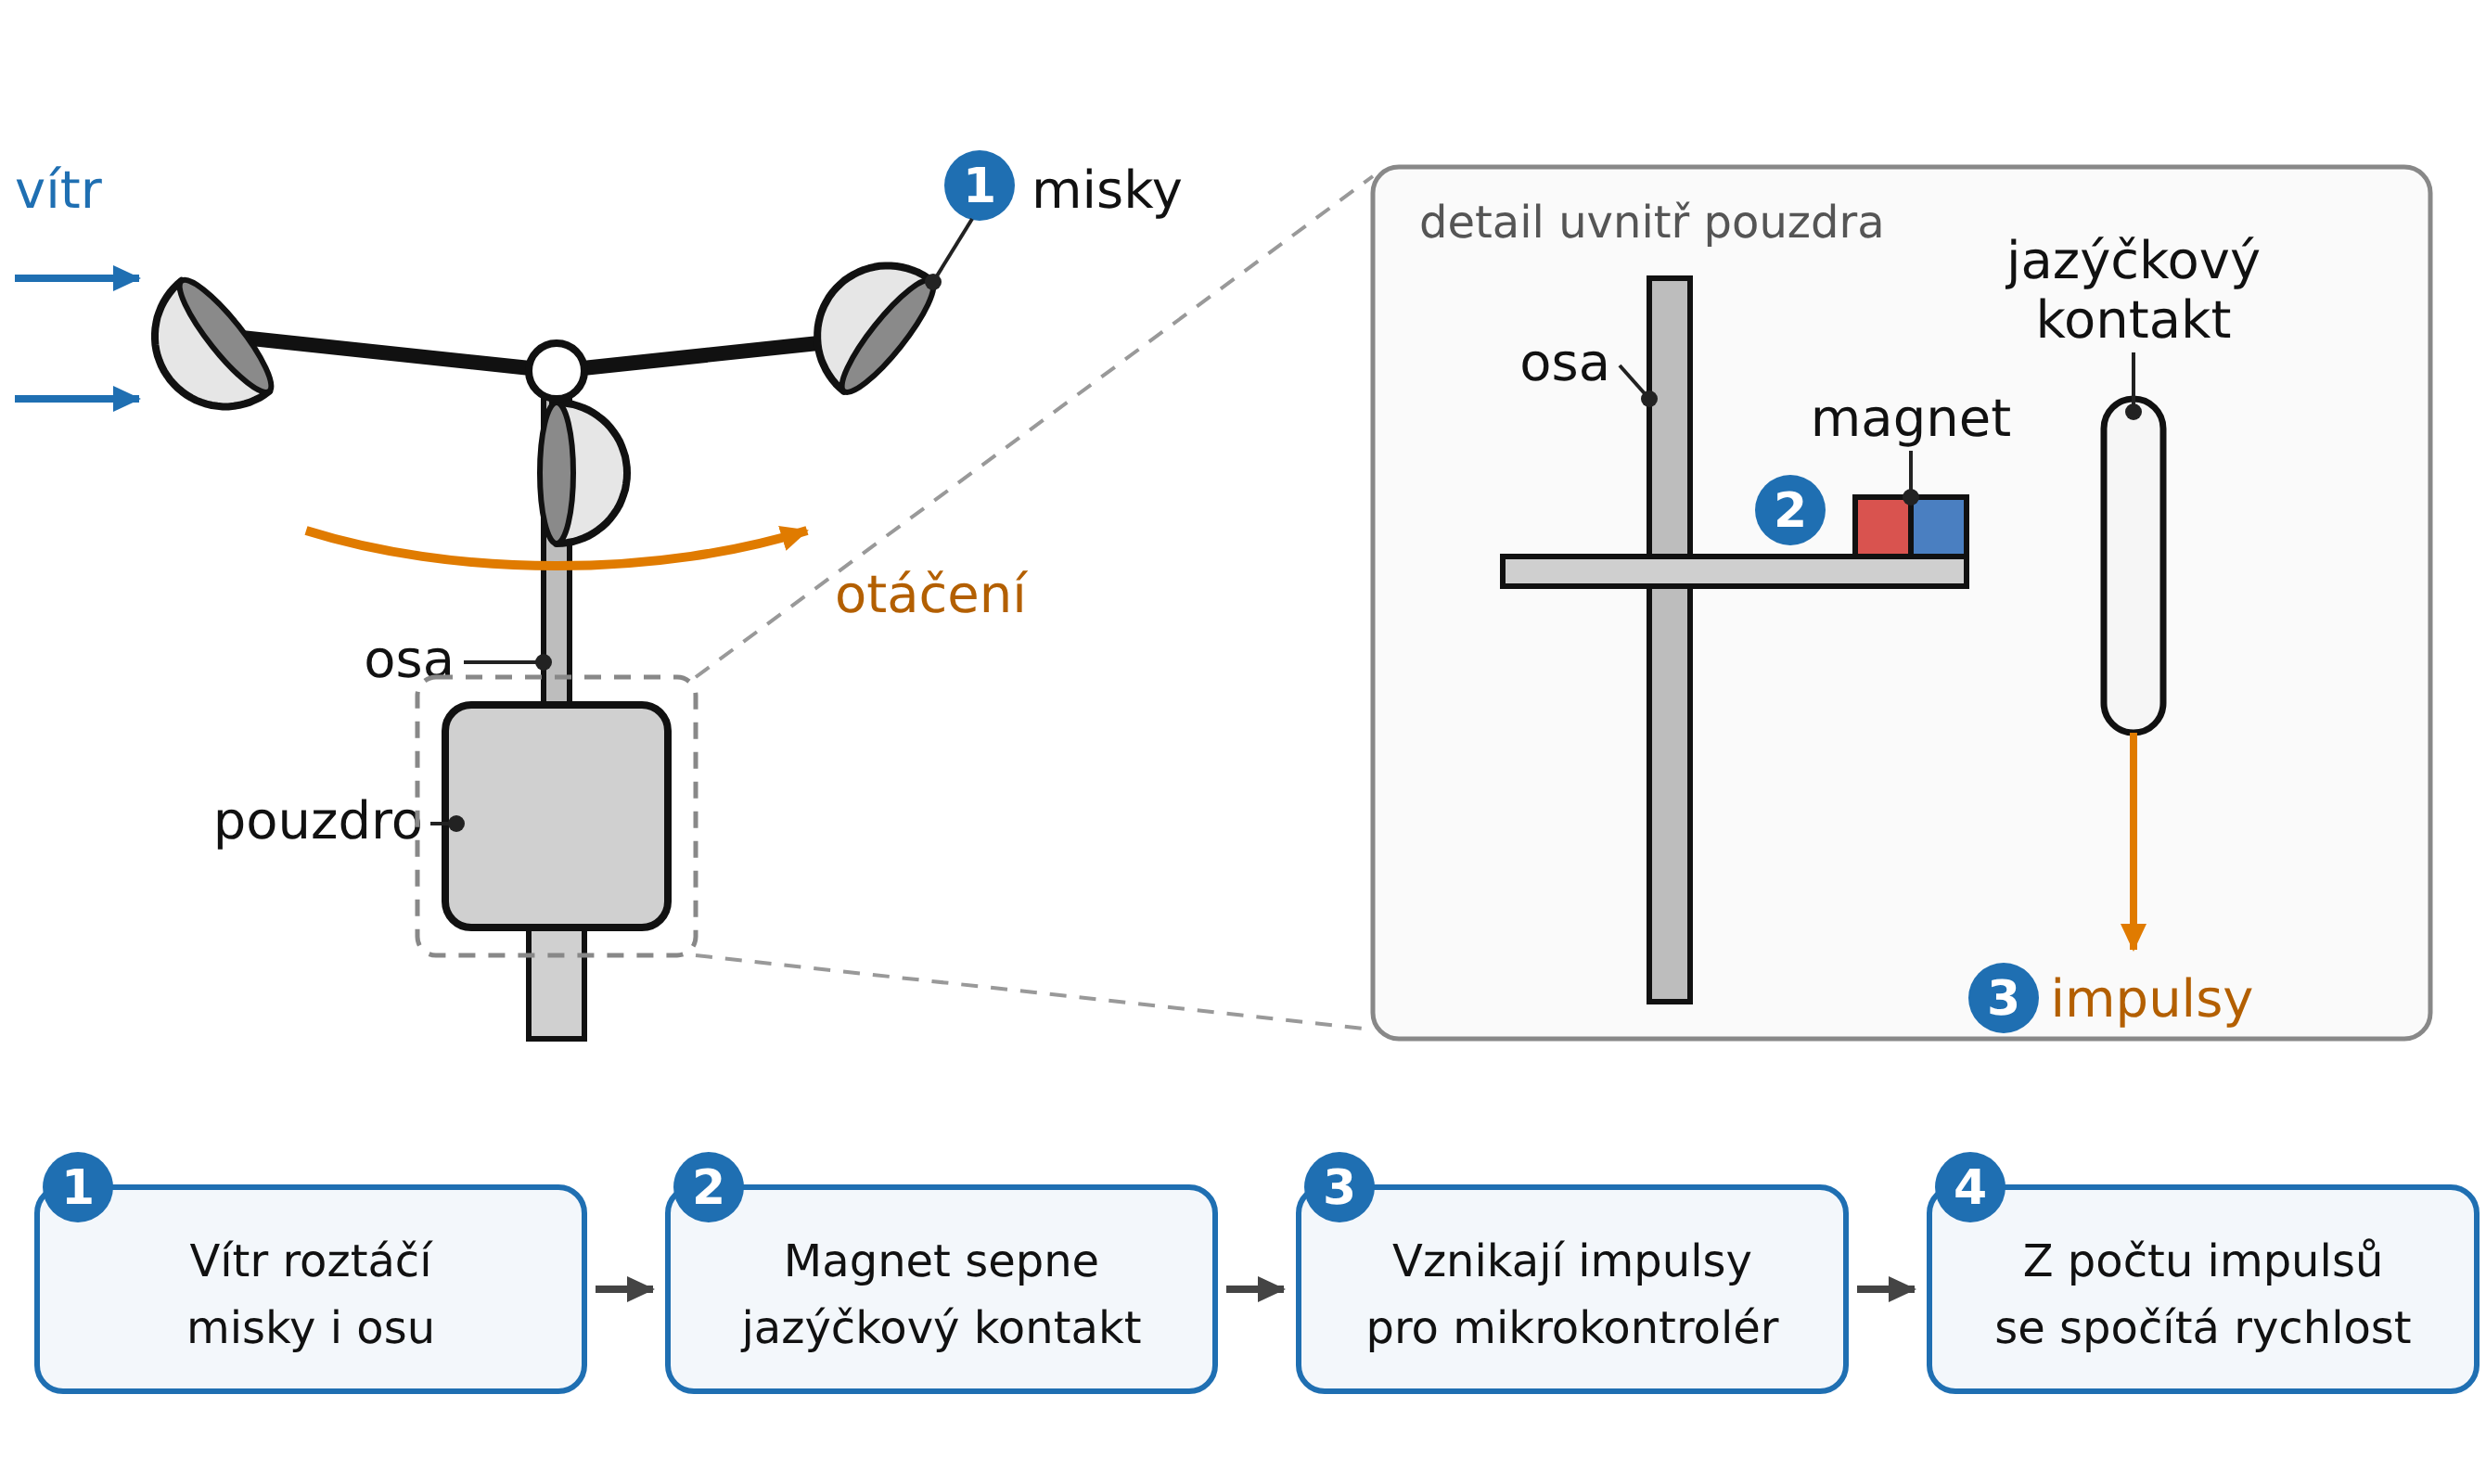
\includegraphics[width=\textwidth]{miskovy_anemometr}
\caption{Princip miskového anemometru}
\label{fig:anemometr}
\end{figure}

\subsection{Větrná směrovka}

Směrovka se otáčí podle směru větru a~nese magnet. Kolem osy je osm jazýčkových kontaktů, z~nichž každý je zapojený s~jiným odporem. Magnet může sepnout jeden kontakt nebo dva sousední najednou, takže vznikne 16~poloh~\cite{sparkfun}. Každá poloha dá na odporovém děliči jiné napětí. To se přečte analogovým vstupem mikrokontroléru a~podle změřené hodnoty se přiřadí ke směru. Dražší čidla používají jiné způsoby snímání a~směr udávají přímo ve stupních.

Princip je znázorněn na obrázku~\ref{fig:smerovka}.

\begin{figure}[htbp]
\centering
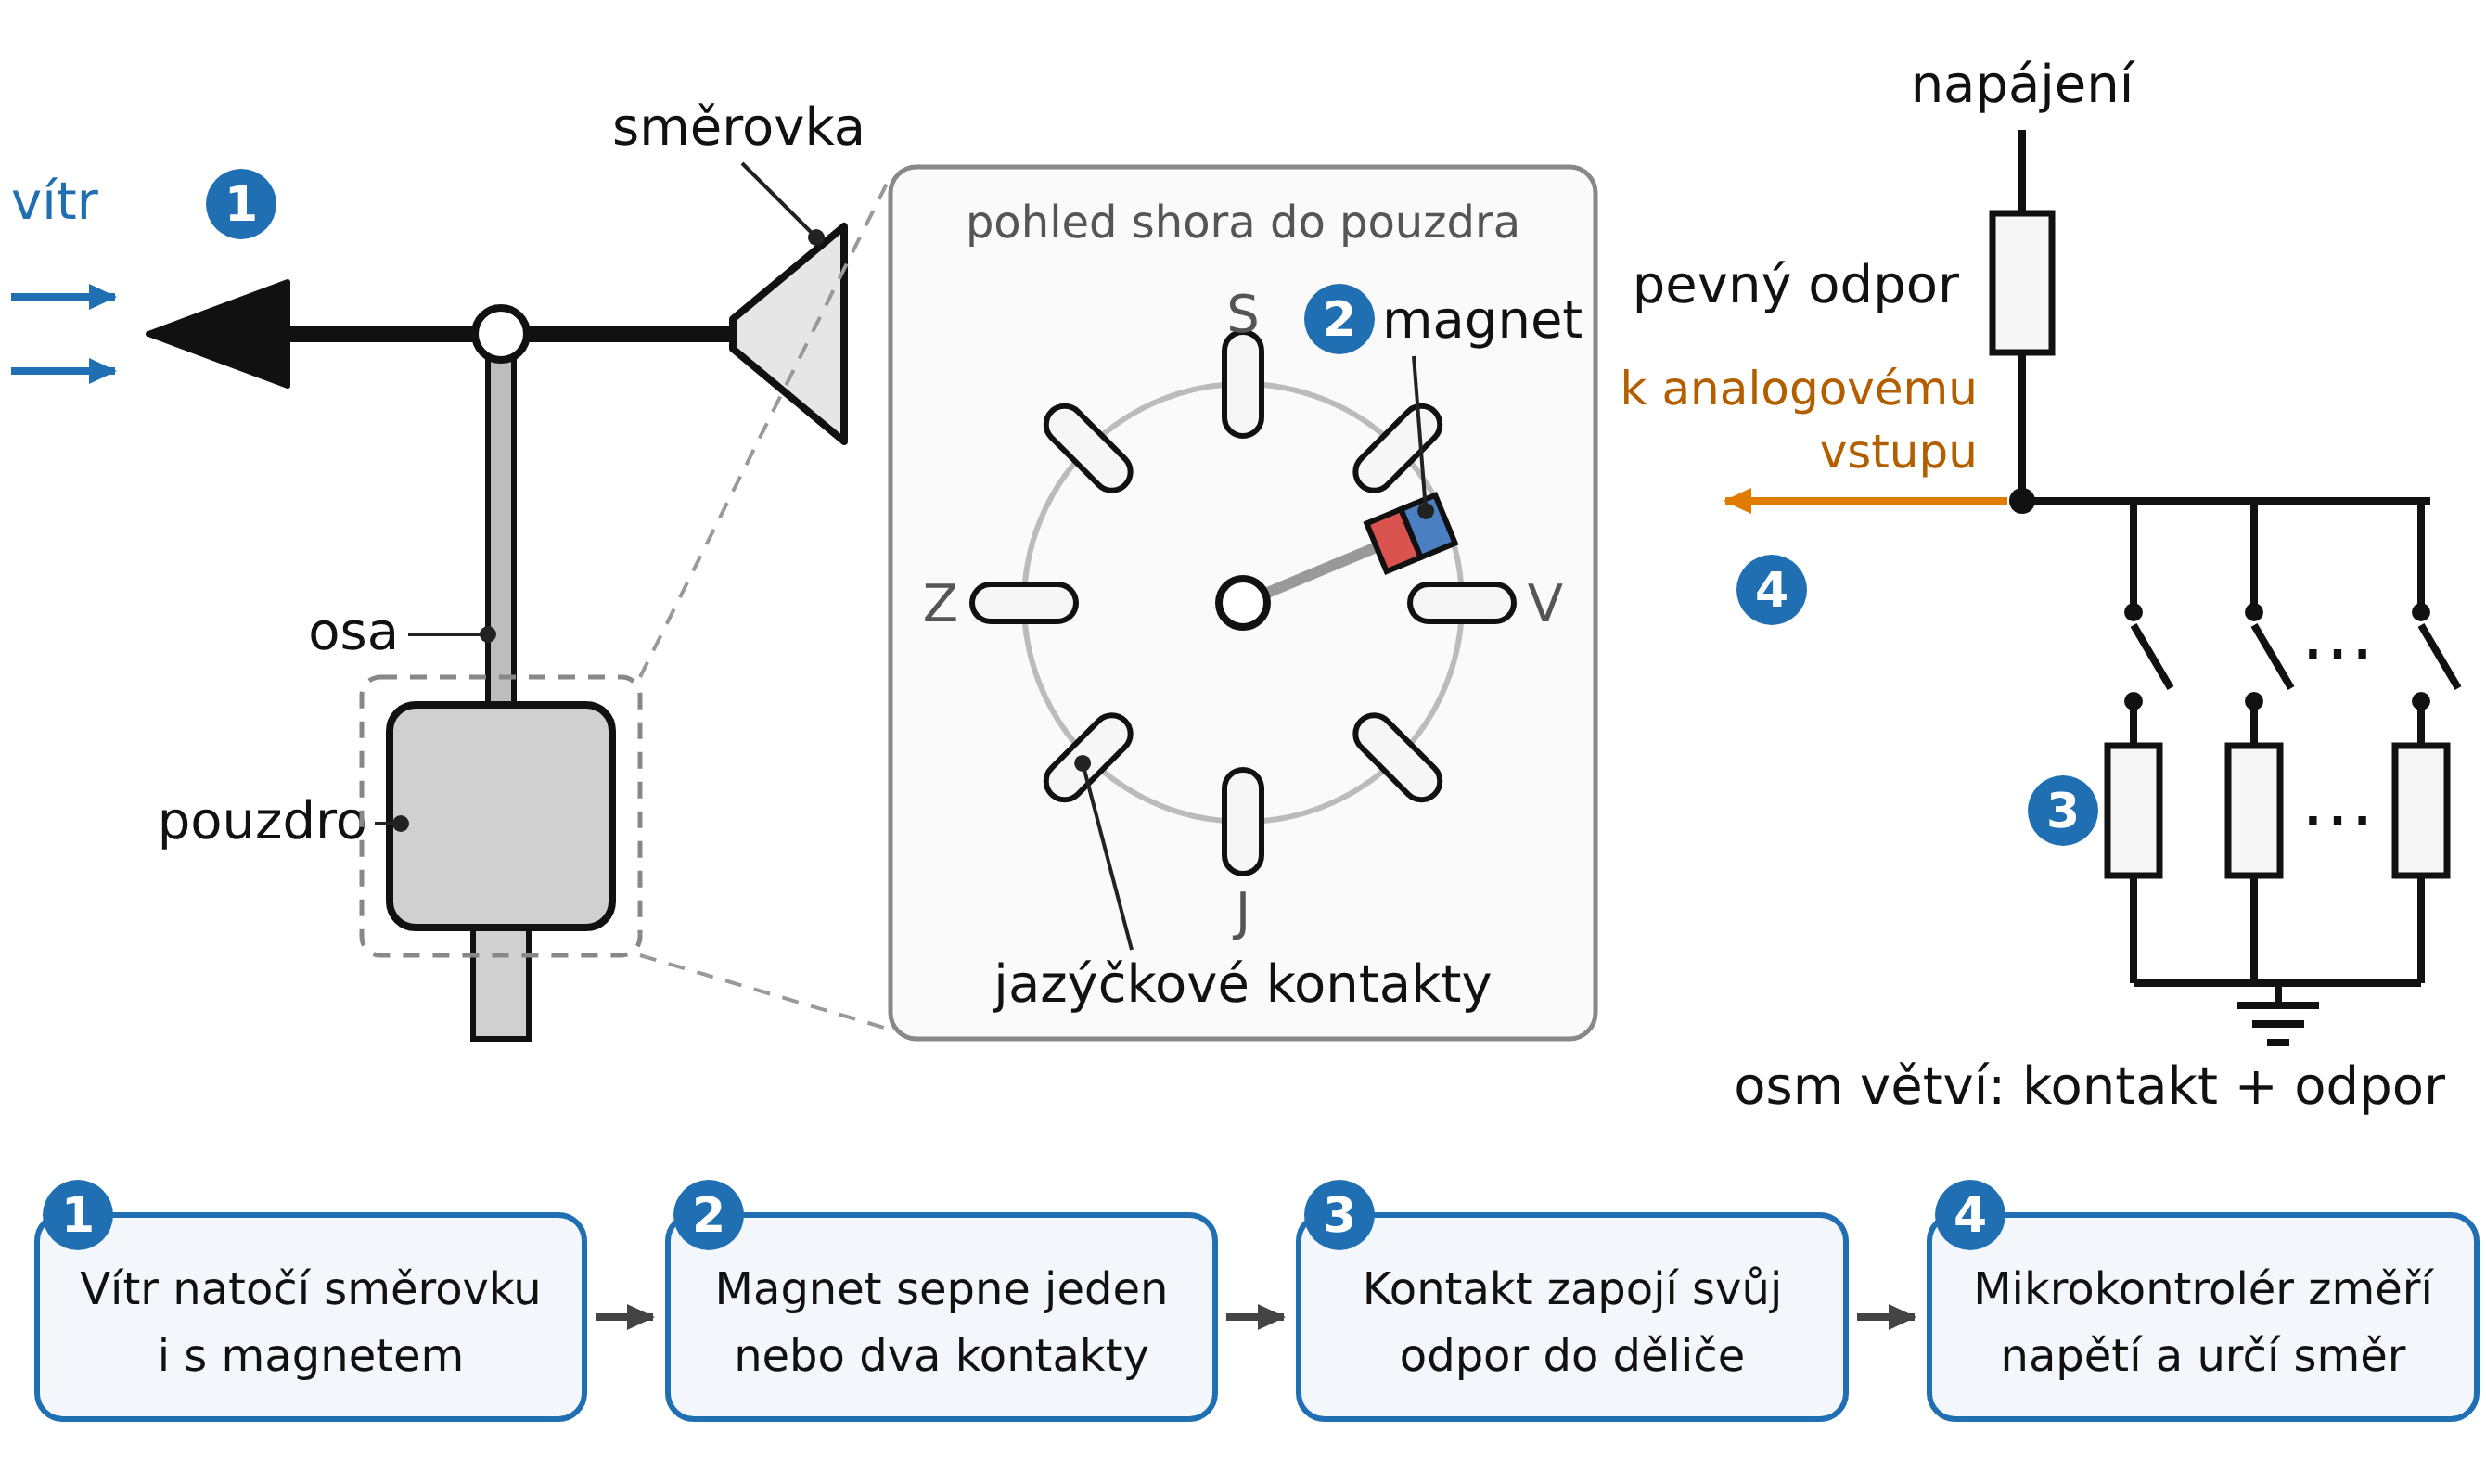
\includegraphics[width=\textwidth]{vetrna_smerovka}
\caption{Princip větrné směrovky s~jazýčkovými kontakty}
\label{fig:smerovka}
\end{figure}

\subsection{Ultrazvukový anemometr}

Ultrazvukový anemometr nemá žádné pohyblivé části. Mezi několika páry měničů posílá krátké ultrazvukové pulzy a~měří, o~kolik se změní doba letu proti větru a~po větru. Z~rozdílu časů se spočítá rychlost i~směr najednou. Výstup bývá digitální, takže je potřeba řešit i~komunikaci s~čidlem.

\subsection{Vrtulkový anemometr}

Vrtulkový anemometr má vrtuli na vodorovné ose a~otáčí se proti větru, takže měří rychlost i~směr jedním čidlem. Používá se hlavně u~profesionálních stanic a~na letištích, proto se mu dál nevěnuji.

\section{Porovnání řešení}

Tabulka~\ref{tab:vitr} shrnuje tři řešení, ke kterým jsem našel dokumentaci. Údaje jsou převzaté z~katalogů a~datasheetů výrobců.

\begin{center}
\noindent\begin{minipage}{\textwidth}
\captionof{table}{Porovnání konkrétních řešení měření větru}
\label{tab:vitr}
\scriptsize
\renewcommand{\arraystretch}{1.25}
\begin{tabularx}{\textwidth}{|Y{1.2}|Y{0.8}|Y{1.1}|Y{0.9}|}
\hline
\textbf{Řešení} & \textbf{Rozsah} & \textbf{Přesnost} & \textbf{Výstup} \\
\hline
\rowcolor{gray!15}\multicolumn{4}{|l|}{\textbf{Miskový anemometr a~směrovka}} \\
\hline
Fine Offset / Misol (anemometr + směrovka) & 0 až 50~m/s & $\pm$1~m/s do 10~m/s, nad tím $\pm$10~\% & kontakt, odporový dělič \\
\hline
Rika RK100-01 + RK110-01 & 0 až 30~m/s & $\pm(0{,}3+0{,}03\,V)$~m/s, směr $\pm$3$^\circ$ & impulsy, napětí, 4--20~mA, RS485 \\
\hline
\rowcolor{gray!15}\multicolumn{4}{|l|}{\textbf{Ultrazvukový}} \\
\hline
Calypso ULP & 0 až 25 nebo 0 až 45~m/s & 1~\% při 10~m/s, směr $\pm$1$^\circ$ & sériový výstup, Modbus \\
\hline
\end{tabularx}

\vspace{0.3em}
{\scriptsize
Poznámky: rozsah a~přesnost u~Fine Offset jsou údaje výrobce pro jeho stanici WH3080, která používá stejný typ čidel. U~Riky je $V$ naměřená rychlost větru v~m/s. Zdroje:~\cite{fineoffset,misolwd,rikawind,rikadir,calypso}.\par}
\end{minipage}
\end{center}

	% Sem vlož seznam použitých zdrojů
\begin{thebibliography}{99}

\bibitem{sparkfun} SPARKFUN ELECTRONICS. \textit{Weather Meter SEN-15901: Datasheet DS-15901} [online]. [cit. 2026-10-23]. Dostupné z: \url{https://cdn.sparkfun.com/assets/d/1/e/0/6/DS-15901-Weather_Meter.pdf}

\bibitem{misol} MISOL. \textit{WH-SP-RG Rain Gauge: Instruction Manual} [online]. [cit. 2026-10-23]. Dostupné z: \url{https://manuals.plus/asin/B00QDMBXUA}

\bibitem{macek} MACEK, Jan. \textit{Domácí meteostanice} [online]. Brno, 2023 [cit. 2026-11-02]. Diplomová práce. Vysoké učení technické v Brně, Fakulta elektrotechniky a komunikačních technologií. Vedoucí práce Soňa Šedivá. Dostupné z: \url{https://theses.cz/id/w5sa8s/Diplomova_prace_-_Jan_Macek.pdf}

\bibitem{ott} OTT HYDROMET. \textit{OTT Pluvio$^2$ S: Data sheet} [online]. [cit. 2026-10-23]. Dostupné z: \url{https://ott.com/download/data-sheet-ott-pluvio-2s-en}

\bibitem{hx711} AVIA SEMICONDUCTOR. \textit{HX711: 24-Bit Analog-to-Digital Converter (ADC) for Weigh Scales} [online]. [cit. 2026-10-23].

\bibitem{cnx} CNX SOFTWARE. \textit{Industrial-grade optical rain gauge beams infrared light to measure rainfall} [online]. 2020 [cit. 2026-10-23]. Dostupné z: \url{https://www.cnx-software.com/2020/07/29/industrial-grade-optical-rain-gauge-beams-infrared-light-to-measure-rainfall/}

\bibitem{rg15} HYDREON. \textit{RG-15 Optical Rain Gauge: Specifications} [online]. [cit. 2026-10-23]. Dostupné z: \url{https://www.mouser.com/datasheet/2/744/RG_15_c2_a0specifications-1890313.pdf}

\bibitem{hestore} HESTORE HUNGARY KFT. \textit{WH-SP-RG: Rain level meter (rain gauge), reed pulse output} [online]. [cit. 2026-10-23]. Dostupné z: \url{https://www.hestore.eu/en/prod_10042313.html}

\bibitem{davis} DAVIS INSTRUMENTS. \textit{Rain Collector 6464/6466: Datasheet} [online]. [cit. 2026-10-23]. Dostupné z: \url{https://www.bmc.de/datenblaetter/DS6464_6466_SS.pdf}

\bibitem{rika} RIKA SENSOR. \textit{RK400-01 Tipping bucket rainfall sensor specification, v5.02} [online]. [cit. 2026-10-23]. Dostupné z: \url{https://img.yfisher.com/m6041/1757578680326-rk400-01-02mmtipping-bucket-rainfall-sensor-specification-v502.pdf}

\bibitem{veinasa} SICHUAN WEINASA TECHNOLOGY. \textit{Veinasa-YL Stainless Metal Digital Tipping Bucket Rain Gauge Sensor} [online]. [cit. 2026-10-23]. Dostupné z: \url{https://e1be750316294ad1.en.made-in-china.com/product/enurLycYYKhA/China-Veinasa-Yl-Stainless-Metal-Digital-Tipping-Bucket-Rain-Gauge-Sensor.html}

\bibitem{bgt} BGT HYDROMET. \textit{High-precision Pulse Siphonic Tipping Bucket Rain Gauge WS-601} [online]. [cit. 2026-10-23]. Dostupné z: \url{https://www.bgt-hydromet.com/high-precision-pulse-siphonic-tipping-bucket-rain-gauge.html}

\bibitem{renkeopt} E-POWER SERVICE. \textit{Renke Optical Rain Gauge} [online]. [cit. 2026-10-23]. Dostupné z: \url{https://www.epower.co.th/product/57820-77952/renke-optical-rain-gauge}

\bibitem{misolwd} MISOL. \textit{WH-SP-WD and WH-SP-RG manual} [online]. [cit. 2026-11-02]. Dostupné z: \url{https://manuals.plus/ae/1005005214339792}

\bibitem{fineoffset} FINE OFFSET ELECTRONICS. \textit{WH3080 Professional Weather Station} [online]. [cit. 2026-11-02]. Dostupné z: \url{https://www.foshk.com/weather_professional/wh3080.html}

\bibitem{rikawind} RIKA SENSOR. \textit{RK100-01 Wind Speed Sensor Specification v3.0} [online]. ESIS Australia [cit. 2026-11-02]. Dostupné z: \url{https://www.esis.com.au/wp/wp-content/uploads/2020/10/RK100-01-wind-speed-specification-v3.0-ESIS-AU.pdf}

\bibitem{rikadir} RIKA SENSOR. \textit{RK110-01 Metallic Wind Direction Sensor (Pulse)} [online]. Instrument Choice [cit. 2026-11-02]. Dostupné z: \url{https://www.instrumentchoice.com.au/products/rk110-01-metallic-wind-direction-sensor-pulse}

\bibitem{calypso} CALYPSO INSTRUMENTS. \textit{Ultra Low Power Ultrasonic Wind Meter} [online]. NauticExpo [cit. 2026-11-02]. Dostupné z: \url{https://pdf.nauticexpo.com/pdf/calypso-marine-instruments/ultra-low-power-ultrasonic-wind-meter/66232-126983.html}

\end{thebibliography}
\end{document}